\documentclass[review]{elsarticle}

\usepackage{lineno,hyperref}
\modulolinenumbers[5]
\usepackage{epstopdf}

\journal{Solar Energy}

%%%%%%%%%%%%%%%%%%%%%%%
%% Elsevier bibliography styles
%%%%%%%%%%%%%%%%%%%%%%%
%% To change the style, put a % in front of the second line of the current 
%style and
%% remove the % from the second line of the style you would like to use.
%%%%%%%%%%%%%%%%%%%%%%%

%% Numbered
%\bibliographystyle{model1-num-names}

%% Numbered without titles
%\bibliographystyle{model1a-num-names}

%% Harvard
%\bibliographystyle{model2-names.bst}\biboptions{authoryear}

%% Vancouver numbered
%\usepackage{numcompress}\bibliographystyle{model3-num-names}

%% Vancouver name/year
%\usepackage{numcompress}\bibliographystyle{model4-names}\biboptions{authoryear}

%% APA style
%\bibliographystyle{model5-names}\biboptions{authoryear}

%% AMA style
%\usepackage{numcompress}\bibliographystyle{model6-num-names}

%% `Elsevier LaTeX' style
\bibliographystyle{elsarticle-num}
%%%%%%%%%%%%%%%%%%%%%%%


\usepackage{geometry}
\usepackage{pdflscape}
\usepackage{supertabular}


\begin{document}

\begin{frontmatter}

\title{Hourly solar power forecasting using ARMA models}
% \tnotetext[mytitlenote]{Fully documented templates are available in the 
% elsarticle package on 
% \href{http://www.ctan.org/tex-archive/macros/latex/contrib/elsarticle}{CTAN}.}

%% Group authors per affiliation:
\author{Bismark Singh}
\address{Discrete Mathematics \& Optimization, Sandia National Laboratories 
\corref{mycorrespondingauthor}}


\author{David Pozo}
\address{Center for Energy Systems , Skolkovo Institute of Science and 
Technology}
%% or include affiliations in footnotes:

\begin{abstract}
We describe a succinct methodology to develop hourly auto-regressive moving 
average (ARMA) models to forecast solar power. We illustrate how to use 
statistical tests to validate the model and construct hourly samples. These 
samples can be used as scenarios for energy planning or in stochastic 
optimization models.
\end{abstract}

\begin{keyword}
ARMA\sep solar energy \sep forecasting \sep scenario generation
\end{keyword}

\end{frontmatter}

\linenumbers

\section{Introduction}
Increasing penetration of renewable energy sources, such as wind and solar, in 
the electricity grid requires good day-ahead power forecasts. Solar power 
differs from wind power due to its diurnal nature, and can have much greater 
ramps than wind~\cite{graabak2016variability}. In this article, we focus 
on forecasting  hourly solar power generation. 

Forecasting methods for solar power are broadly divided 
into two categories: (i) physics-based models---these models predict solar power 
from numerical weather predictions and solar irradiation data, and (ii) statistical models---these 
models forecast 
solar power directly from historical data. Comparisons of these two 
methods are also available; see, 
e.g.,~\cite{huang2010comparative,inman2013solar}. There are other 
approaches available as well which combine these two 
methods~\cite{chen2011online}. 
In this article we center on  statistical  methods alone, and specifically the 
use of auto-regressive moving average (ARMA) 
models to develop our forecasts. ARMA models are widely used for forecasting 
many economic and planning processes; see, e.g.,~\cite{box2008time}. They 
 have also been used to forecast wind power~\cite{brown1984time, 
duran2007short}, as well as solar 
power~\cite{mora1998multiplicative,huang2012solar}.  Yet, accurate and 
fast methods to generate solar power scenarios are often unavailable, and 
normal approximations are often used; see, e.g.,~\cite{su2014stochastic}. Here, 
we describe an  
in-depth summary of the methodology to forecast solar power using ARMA models. 
The presented models can 
be applied either to a local photo-voltaic generating plant or  at the regional 
level.

\section{Methods}
We take hourly year-long historical solar power output 
from~\cite{golestaneh2016generation}. We use approximately nine months of data 
for training. The data does not have any solar power for the ten hours 
[20:00-5:00], and hence we restrict the forecasts in these hours to be zero as 
well. For each of the remaining 14 hours of the day, we build an ARMA$(p,q)$ 
model. Further, for each hour, we verify the stationarity of the time 
series. For each hour, we test a number of ARMA($p,q$) models and find the best 
one. We use statistical tests on the residuals to validate the model. Finally, 
we use Monte Carlo sampling from the best ARMA model, for each hour, to create 
hourly scenarios. Below we provide more details.

\subsection{Stationarity}
An ARMA model may be suitable if a series is stationary. We test 
the hourly data for stationarity using the Augmented 
Dickey-Fuller (ADF) test~\cite{dickey1979distribution}. The ADF test has a null 
hypothesis that the series includes a unit root (or, is non-stationary). We 
reject the null hypothesis at a level 0.05 if the test-statistic exceeds its 
0.95 level quantile. For all the 14 hours of the day, the null hypothesis is 
rejected suggesting the series may be stationary, and hence an ARMA model may 
be suitable. If the series were not stationary, an ARIMA model may be suitable.

\subsection{Selecting parameters of the ARMA model}
Next, we estimate the parameters of the ARMA model---$p$, the order of the 
autoregressive part and, $q$, the order of the moving average part. For each 
hour, we construct 16 models with both $p$ and $q$ between one and four, and 
compute 
the log-likelihood objective function value. Next, for each hour, we calculate 
the Bayesian information criteria (BIC) for the 16 models using $p + q + 1$ 
parameters.  The BIC penalizes for models with more parameters, and the 
smallest value of the BIC gives the best model, for each 
hour. Table~\ref{tab:order} provides our estimated $p$ and $q$  values for 
the 14 hours of the day. We note that none of the hours have an order value 
exceeding two.

\begin{table}[!htb]
\centering
\caption{Estimated $p$ and $q$ values for ARMA($p,q$) models for 14 hours of 
the day}
\label{tab:order}
\scalebox{0.8}{
\begin{tabular}{c| cccccccccccccc}
\hline 
Hour & 6:00 & 7:00 & 8:00 & 9:00 & 10:00 & 11:00 & 12:00 & 13:00 & 14:00 
& 15:00 & 16:00 & 17:00 & 18:00 & 19:00 \\ \hline
p    & 1    & 1    & 1    & 1    & 2     & 1     & 1     & 1     & 1     & 1     
& 1     & 1     & 1     & 2     \\ \hline
q    & 1    & 1    & 1    & 1    & 1     & 1     & 2     & 1     & 1     & 1     
& 1     & 1     & 2     & 1   
\end{tabular}}
\end{table}

\subsection{Prediction}

Figure~\ref{fig:prediction} plots a day-ahead prediction using the above 
constructed ARMA models; i.e., one hour ahead predictions from the 14 ARMA 
models. The mean absolute error between the actual and the predicted series is 
39.6, or  3.3\% of the maximum actual value. The root mean square 
error between the actual and the predicted series is 
61.0, or  5.1\% of the maximum actual value. 

We further verify autocorrelation in the series, for each hour, using the 
Ljung-Box test~\cite{ljung1978measure} on the residuals for lags of 5, 10, 
and 15. The Ljung-Box  test has a 
null hypothesis that the residuals are uncorrelated up to a 
given lag. We reject the null hypothesis at a level 0.05 if its test-statistic 
exceeds its 
0.95 level quantile. For all the 14 hours of the day, the null hypothesis is not
rejected suggesting a zero autocorrelation in the series, or the 
model choice may be appropriate. 


\begin{figure}[!t]
\centering
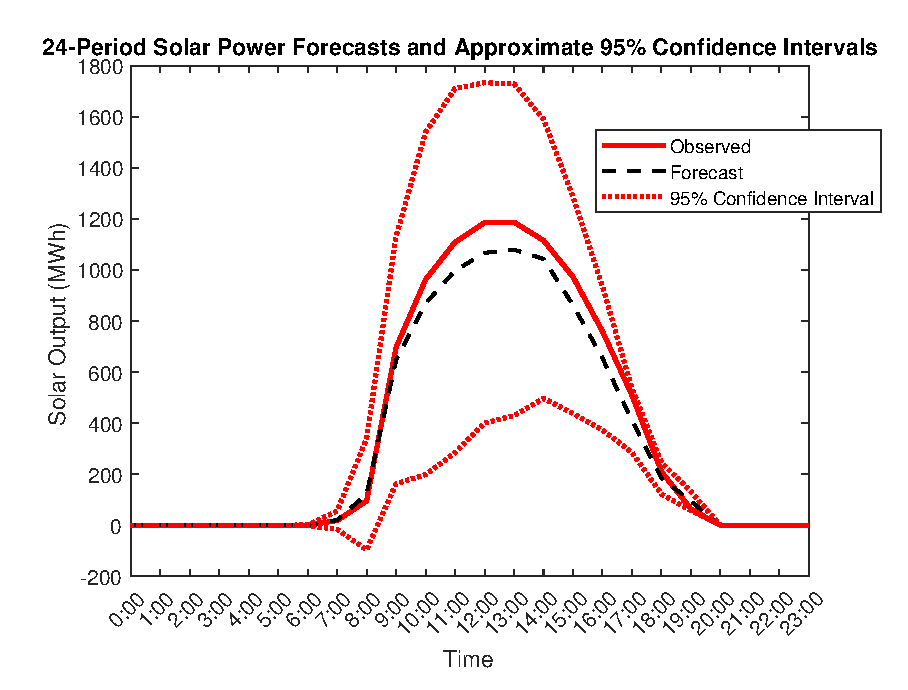
\includegraphics[width=0.8\textwidth]{prediction.eps}
\caption{Day-ahead actual and predicted values using ARMA models from 
Table~\ref{tab:order}}
 \label{fig:prediction}
\end{figure}

Finally, we use Monte Carlo sampling to generate 2000 hourly solar power 
scenarios. The output from an ARMA model is real valued, and hence can be 
negative. We truncate the negative powered outputs to 0. For the 14 hours of 
the day, the sampling resulted in 1.6\% of the outputs with estimated power 
output below -5MWh. Figure~\ref{fig:sample} plots the 2000 day-ahead scenarios 
as well as the median and 10 percentile values. 


\begin{figure}[!t]
\centering
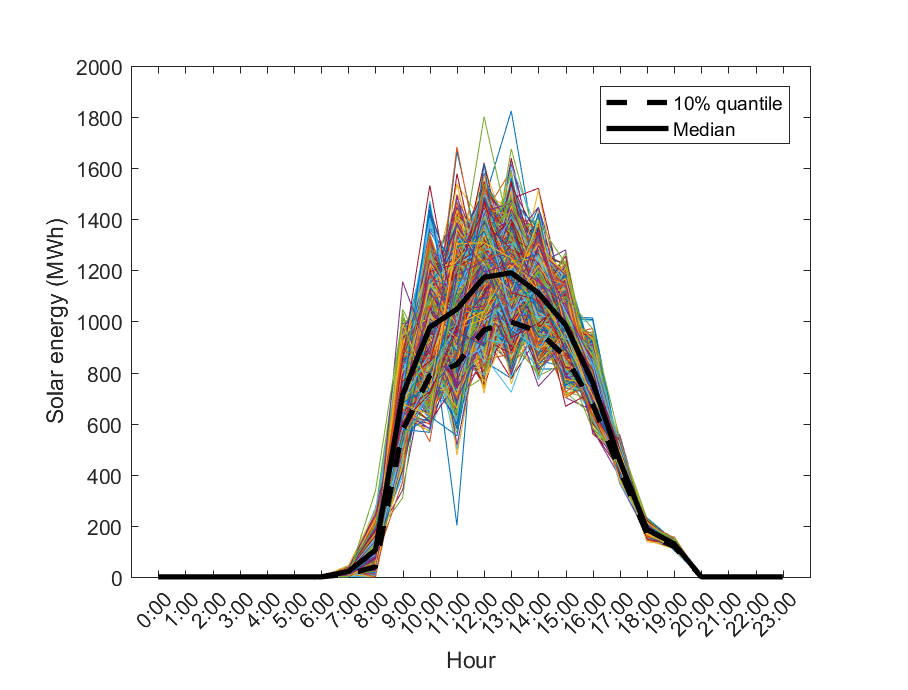
\includegraphics[width=0.9\textwidth]{sample_smooth.eps}
\caption{2000 hourly scenarios for solar power generated using the ARMA models 
from Table~\ref{tab:order}. The dashed black line is the median hourly value, 
and the solid black line is
the 10 percentile solar energy value.}
 \label{fig:sample}
\end{figure}

\section*{Conclusions}
We present a step-by-step methodology for fitting an ARMA model to 
historical solar power data, and use it to forecast future hourly scenarios. We 
present statistical tests to check the applicability of the model and 
investigate the fit, at each step. This methodology can be directly applied to 
historical data to analyze if an ARMA model might be suitable, and can be used 
to create future scenarios for use in a stochastic model.


\section*{Acknowledgments} 
The authors thank Jean-Paul Watson and Andrea Staid at Sandia National 
Laboratories for helpful discussions and for sharing data. 
Sandia National Laboratories is a multimission laboratory managed and operated 
by National Technology and Engineering Solutions of Sandia, LLC., a wholly owned
subsidiary of Honeywell International, Inc., for the U.S. Department of 
Energy's 
National Nuclear Security Administration under contract DE-NA-0003525.

\section*{References}

\bibliography{mybibfile}

\end{document}